\noindent
\subsection{Editor}
\label{editor}   

\begin{figure}
\centering
\includegraphics*[width=.48\textwidth]{figures/editor_all.eps}
\caption{\label{fig3}(a) Median Average citation (MAC) versus $MEAT$. $MEAT$ values are bucketed into 12 bins of equal size with range(1, 498.8).(b) MAC versus $SRI$ and (c) MAC versus $RADI$. For both (b) and (c), the x-axis values are bucketed by values corresponding to ($\geq$ 0 and $<$ 0.1), ($\geq$ 0.1 and $<$ 0.2) and so on.}
\end{figure}

\begin{figure}[!ht]
\centering
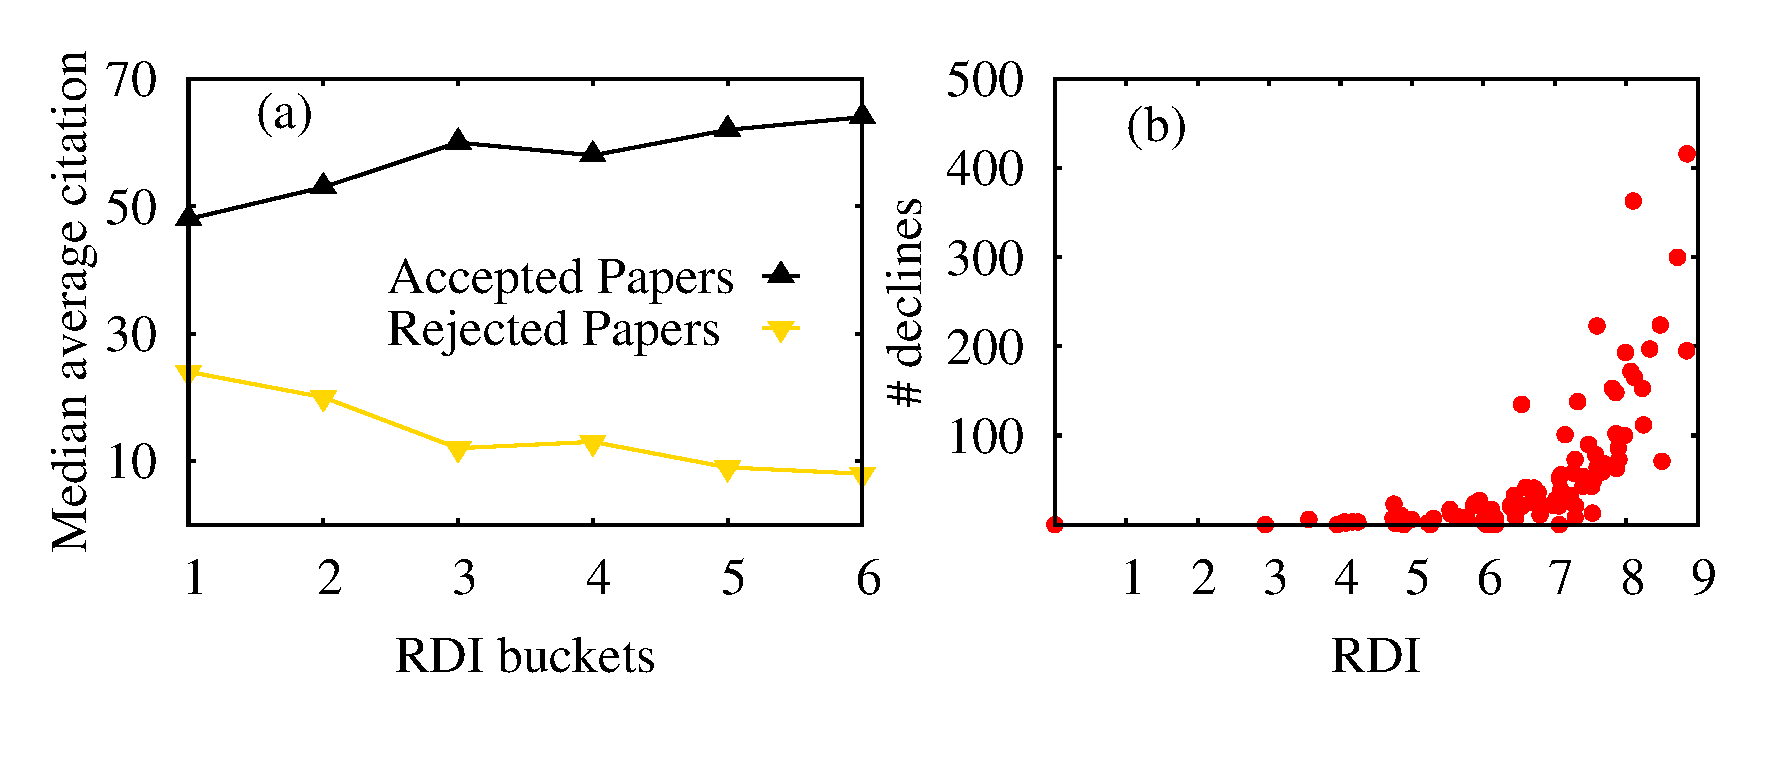
\includegraphics[scale=0.27]{figures/RDI_RDI_diversity.eps}
\caption{\label{fig_sri} (a) Median Average citation versus $SRI$. $SRI$ values are bucketed by values corresponding to ($\geq$ 0 and $<$ 0.1), ($\geq$ 0.1 and $<$ 0.2) and so on. (b) $RDI$ versus number of declines. Increasing trend indicates higher the $RDI$, higher is the number of declines.}
\end{figure}

\begin{figure}[!ht]
\centering
\includegraphics*[width=0.48\textwidth]{figures/reviewer_all.eps}
\caption{\label{fig5}(a) Median Average citation (MAC) versus $MRAT$. $MRAT$ values are bucketed into 20 buckets of equal size with range(1,498.8),(b) MAC versus $MRSD$ (c) MAC versus $TDI$, (d) MAC versus $EDI$, (e) MAC versus $MTD$ and (f) MAC versus $AR$. For both (c),(d) and (e), the x-axis values are bucketed by values corresponding to ($\geq$ 0 and $<$ 0.1), ($\geq$ 0.1 and $<$ 0.2) and so on. For (b) and (f) values (x-axis) are divided into 10 buckets of equal size.}
\end{figure}

We begin by analyzing the anomalous behavior of the editors. We define the behavior of an editor to be anomalous if the papers assigned to her are on average cited less when accepted or are cited more when rejected. In specific, we investigate different factors related to the editor that can lead to such anomaly.
\subsubsection{Mean Editor Assignment Time (MEAT)}
For each editor we obtain the time span (in days) between any two consecutive assignments and calculate the average time span between the two assignments. 
%The main objective is to check whether an editor who is assigned less frequently does a better job than an editor who is assigned more frequently. 
Formally, we define for editor $i$, $MEAT_{i}$ as
\begin{center}
$MEAT_{i}=\frac{1}{n-1}\sum (\delta_{j+1} - \delta_{j})$
\end{center}
where $n$ is the total number of assignments to the editor $i$ and $\delta_{j}$ is the date of the $j$$^\textrm{th}$ assignment. 
In figure~\ref{fig3}(a) we bin the editors based on the $MEAT$ and calculate the median average citation of the papers assigned to the editors in each bin. 
{We observe that for accepted papers very low or very high $MEAT$ values lead to lower citations. An exact opposite behavior is observed for rejected papers. 
This indicates that editors who are assigned time and again (low $MEAT$) or rarely (high $MEAT$) often fail to judge the quality of the papers assigned to them.} 
%Citation increases as $MEAT$ value increases which is then followed by decrease {\bf Not Clear} indicating that editors who are assigned very less frequently are also anomalous. 

\subsubsection{Self Review Index (SRI)}

%In many cases an editor assigns himself as a reviewer instead of assigning a different referee. While in some of these cases she could not find a reviewer (the reviewer declined), in many other cases she did not try to find a reviewer in the first place. 
{\bf Self Review Index (SRI)} measures the fraction of papers for which the editor assigned herself as the reviewer. 
Formally, for an editor $i$, we define $SRI_{i}$ as 
\begin{center}
$SRI_{i}=\frac{\varrho_{i}}{\rho_{i}}$
\end{center}
where $\rho_{i}$ is the number of papers $i$ was assigned as editor while $\varrho_{i}$ is the number of papers $i$ assigned herself as reviewer. We observe that with increasing values of $SRI$ the median average citation for accepted papers decreases while that for rejected papers increases (refer to figure \ref{fig3}(b)). 

\subsubsection{Referee-Author pair Diversity Index (RADI)}

We observe that editors in numerous cases assign papers from a certain author to only a certain reviewer. To investigate whether this allows for less impactful research from this author getting accepted, we define a metric which we call {\bf Referee-Author pair Diversity Index (RADI)}. Formally we define for editor $i$, the $RADI_{i}$ score as 

\begin{center}
$RADI_{i}=-\sum \limits_{j,k} p_{j,k} \log p_{j,k}$
\end{center}

where $p_{j,k}$ denotes the proportion of times a paper from author $k$ was assigned to reviewer $j$ by the editor $i$. In figure~\ref{fig3}(c) we bin the editors based on the $RADI$ and calculate the median average citation of the papers assigned to the editors in each bin. We observe that more the diversity score higher is the citation of the accepted papers and correspondingly lower is the citation of the rejected papers.


%[{\color{red}{\bf Check the last line; I have changed it. What you wrote earlier was not correct.}}]

\subsubsection{Referee Diversity Index (RDI)}
As a following step, we check whether an editor always chooses from a fixed set of reviewers or a diverse set of reviewers while making a paper assignment and, more importantly, does this influence the performance of the editor in terms of the impact of the reviewed paper. We define for each editor($i$) a metric called {\bf Referee Diversity Index ($RDI_{i}$)} as -  
%which assigns a diversity score for each reviewer depending on whether she selects from a diverse set of reviewers or a small fixed set while assigning. Formally for an editor $i$, $RDI_i$ is defined as
\begin{center}
$RDI_{i}=-\sum \limits_{j} p_{j}\log p_{j}$
\end{center}
where $p_{j}$ denotes the proportion of times reviewer $j$ was assigned a paper by editor $i$. More diverse the set of reviewers higher is the score. In figure~\ref{fig3}(b) we bin the editors based on the $RDI$ and calculate the median average citation of the papers assigned to the editors in each bin. We observe that more the diversity score, higher is the citation of the accepted papers and correspondingly lower is the citation of the rejected papers.

A summary statistic of all the above factors that may be used to identify anomalous editors are noted in Table~\ref{summary_stat}.

%\subsubsection*{Pathological cases}
The dataset allows us to find out the cases when the reviewer declined to review a paper on being assigned by an editor. We observe that editors with high $RDI$ are also declined more often. In figure~\ref{fig_sri}(b) we plot $RDI$ value and the number of declines for each editor. An increasing trend indicates that more diversely the editor tries to select reviewers more she gets declined by the reviewers. This in many cases may force the editor to be less proactive and always select from a specific set of `reliable' referees.  

%\subsubsection*{Pathological cases}

%We further looked into some pathological cases which are summarized below - \\
%(i) There are {\bf 1598} submissions which were initially rejected and then successfully appealed by the authors for reconsideration. {\bf 48.72\%} of these were finally accepted, while rest of them were either rejected or withdrawn by the authors. An important observation is that in {\bf 19.8\%} of the cases the paper was again assigned the same editor while for the rest a new editor was assigned. Another surprising observation is that in the {\bf 45.6\%} of the cases where the paper was finally accepted, it was assigned to a specific editor.\\
%(ii) There are {\bf 4006} papers that were declined at least once by a reviewer before being reviewed. We observed that the papers which were declined more than once tend to be low cited on average.
%\begin{figure}
%\centering
%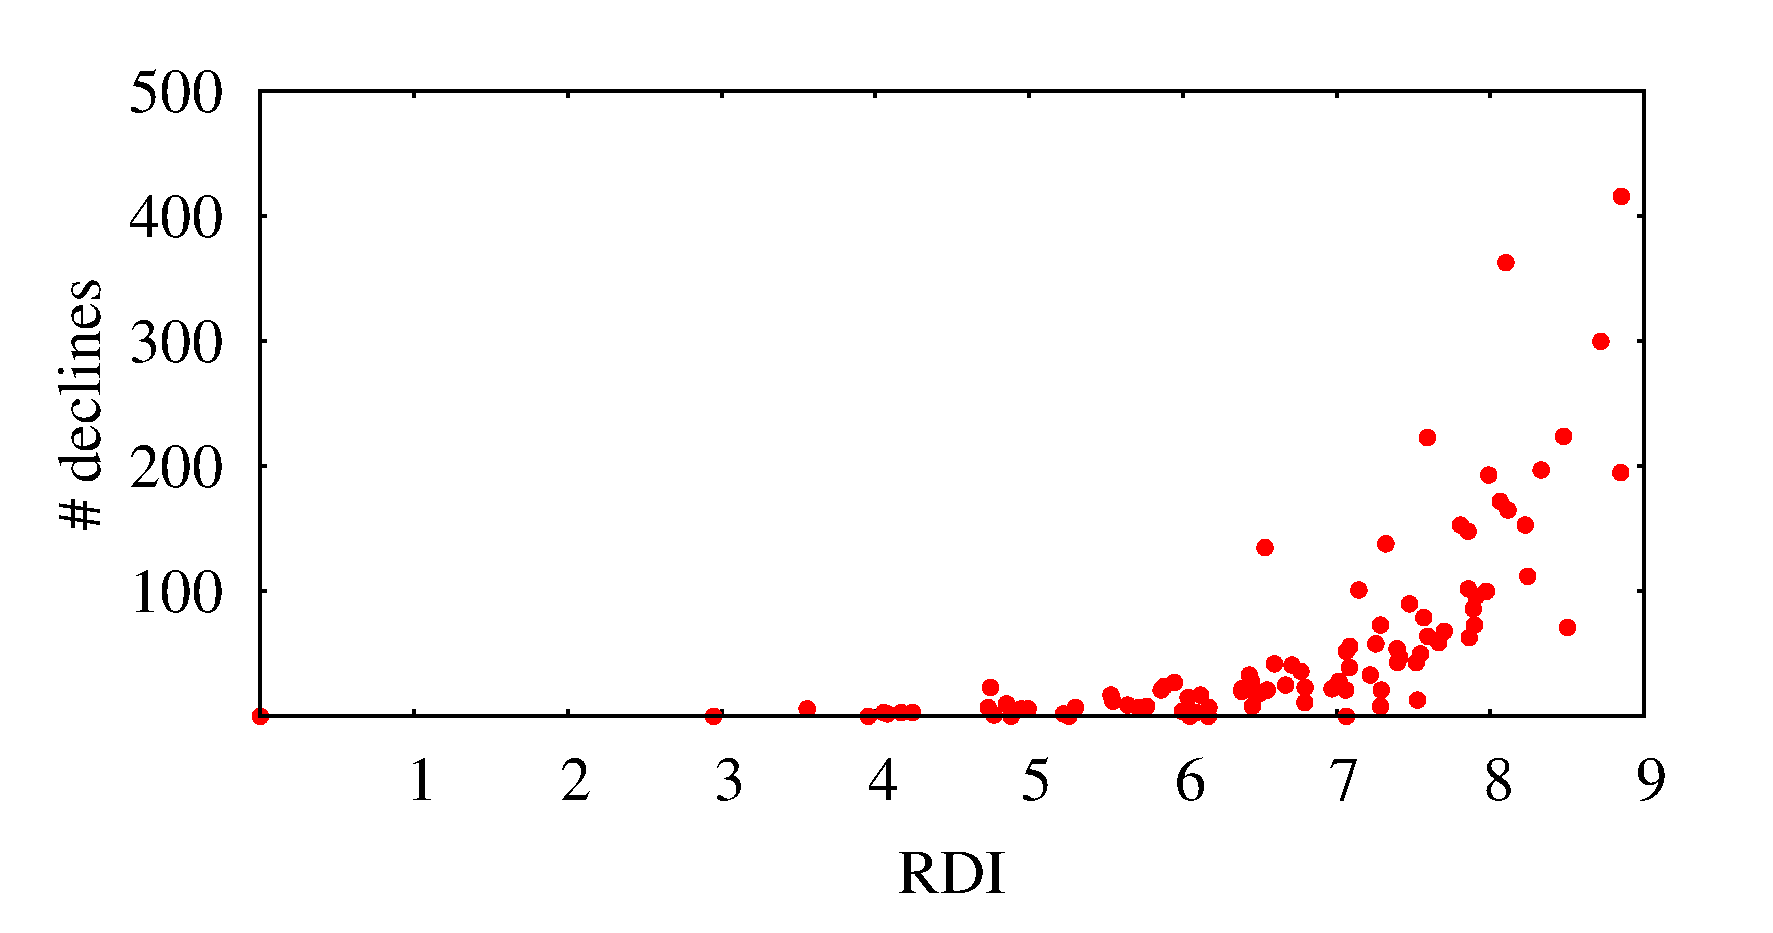
\includegraphics[scale=0.23]{figures/div_decline.eps}
%\caption{\label{fig4} $RDI$ versus number of declines. Increasing trend indicates higher the $RDI$, higher is the number of declines.}
%\end{figure}